\documentclass{article}
\usepackage[utf8]{inputenc}
\usepackage[margin=2.5cm]{geometry}
\usepackage{listings}
\usepackage{xcolor}
\usepackage{pdflscape}
\usepackage{graphicx}

\lstdefinestyle{customc}{
  belowcaptionskip=1\baselineskip,
  breaklines=true,
  frame=L,
  xleftmargin=\parindent,
  language=C,
  showstringspaces=false,
  basicstyle=\footnotesize\ttfamily,
  keywordstyle=\bfseries\color{green!20!black},
  commentstyle=\itshape\color{purple!40!black},
  identifierstyle=\color{blue},
  stringstyle=\color{orange},
}

\lstset{style=customc, tabsize=4}

\title{Embedded Microcontrollers HET232 \\ Experiment 5}
\author{Daniel Parker \\ 971328X \and Mustafa Rizvi \\ 1754270}
\date{\today}

\begin{document}

\maketitle
\section{Aim}
This experiment aimed to develop an embedded C program to run on the Freescale FRDM-K20D50M MCU with LCD module. The program contains two parts; a clock which utilised the Real-Time Clock (RTC) hardware feature and draws the time in either digital or analog format on the LCD, and a musical alarm which utilises the FlexTimer Module (FTM) to create PWM signals to a piezoelectric speaker. The two parts must utilise interrupts so that they can run concurrently. Each part of the program will be explained separately to the source code and the source can be found in the last section of the report.

\maketitle
\section{Basic Clock}
The basic clock functionality is mostly in the digital\_clock program module, however some of the pin initialisation is done in the main file. The digital clock makes available a few accessor functions to it's module level global variables. These accessors can be seen in the header file digital\_clock.h. The microcontroller's real time clock has been setup to interrupt whenever a second has passed (ie. when the clock ticks). In the \emph{void RTC\_Seconds\_IRQHandler(void)} interrupt handler the new time is output on the LCD. No interrupt flag has to be cleared for this module as per the specifications. The user will be asked to set the time when the program first runs as seen in \emph{void user\_time\_setup(void)} from five\_switch.h and five\_switch.c.

\maketitle
\section{Alarm Function}
The alarm can be set using the 5-way switch on the LCD board in the same way as setting the time. music\_box.h provides interface accessor functions for the other modules to use to change the current note being played. To play sound, the module outputs a square wave by toggling the pin associated with the FlexTimer Module 0 Channel 3. The speed at which this happens is dependent on the half period of the desired wave in timer ticks, which is calculated in this module. Interrupts are scheduled at half periods and the previous interrupt flag is cleared on the channel which interrupted. Channel 7 on the FlexTimer Module is configured to interrupt at set intervals and check whether the current note has been playing long enough. 

\newpage
\begin{figure}
\centering
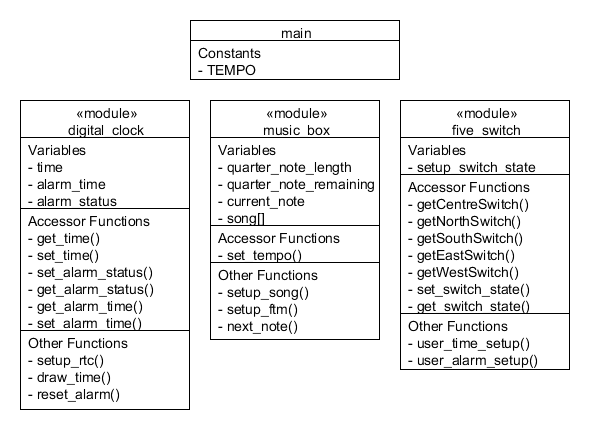
\includegraphics[width=150mm]{module_diagram.png}
\caption{Module Diagram}
\label{overflow}
\end{figure}


\begin{landscape}
\section{source code}
\bf{\underline{main.c}}
\begin{lstlisting}[frame=single]
/*	Digital alarm clock
 * 
 * 	Authors: Daniel and Mustafa
 */

#include <stdio.h>
#include <stdlib.h>
#include "derivative.h"
#include "nokia_LCD.h"
#include "uart.h"
#include "Freedom.h"
#include "digital_clock.h"			// Digital Alarm clock
#include "music_box.h"				// Music Player
#include "five_switch.h"			// 5 way switch control
#include "utilities.h"

#define BACKGROUND_COLOR 	BLACK
#define TEMPO				(140)	// Song Tempo in Beats Per Minute where 1 beat equals a quarter note

/*
 *  Setup code for any physical board pin usage
 */
void setup_pin_hardware(void) {
   // Enable all port clocks (can prune after design finished)
   SIM_SCGC5 |=   SIM_SCGC5_PORTA_MASK
		   	   	| SIM_SCGC5_PORTB_MASK
		   	   	| SIM_SCGC5_PORTC_MASK
		   	   	| SIM_SCGC5_PORTD_MASK;
   
   // Enable FTM and RTC clocks
   SIM_SCGC6 |= SIM_SCGC6_FTM0_MASK | SIM_SCGC6_RTC_MASK;
   
   PORTC_PCR4	= PORT_PCR_MUX(4) | PORT_PCR_DSE_MASK; // Speaker and FTM0_Channel 3
   PORTD_PCR7	= PORT_PCR_MUX(4);
   
   // Setup 5 way switch port options
   CENTRE_SWITCH_PCR   = PORT_PCR_MUX(1)|PORT_PCR_PE_MASK|PORT_PCR_PS_MASK;
   CENTRE_SWITCH_PDDR &= ~CENTRE_SWITCH_MASK;
   
   NORTH_SWITCH_PCR   = PORT_PCR_MUX(1)|PORT_PCR_PE_MASK|PORT_PCR_PS_MASK;
   NORTH_SWITCH_PDDR &= ~NORTH_SWITCH_MASK;   
   
   EAST_SWITCH_PCR   = PORT_PCR_MUX(1)|PORT_PCR_PE_MASK|PORT_PCR_PS_MASK;
   EAST_SWITCH_PDDR &= ~EAST_SWITCH_MASK;
   
   SOUTH_SWITCH_PCR   = PORT_PCR_MUX(1)|PORT_PCR_PE_MASK|PORT_PCR_PS_MASK;
   SOUTH_SWITCH_PDDR &= ~SOUTH_SWITCH_MASK;
   
   WEST_SWITCH_PCR   = PORT_PCR_MUX(1)|PORT_PCR_PE_MASK|PORT_PCR_PS_MASK;
   WEST_SWITCH_PDDR &= ~WEST_SWITCH_MASK;
}


int main(void) {
	int i;
	clock_initialise();				// Clock initialiser for usb debugging messages
	setup_pin_hardware();			// Setup ports and clocks for the timers
	lcd_initialise();				// Initialise LCD
	lcd_clear(BACKGROUND_COLOR);	// Black the LCD

	set_tempo(TEMPO);				// Calculates the relevant tick information for the given tempo
	setup_song();					// Initialises the song
	
	set_switch_state(1);			// Hours set switch mode
	draw_time(get_time());			// Draws 12:00:00
	user_time_setup();				// User can set the initial RTC time
	
	set_alarm_time(get_time());		// Set alarm time to same as main time
	setup_rtc(get_time());			// Turns on the Real-Time Clock
	
	// Wait for user to release the centre switch
	while(getCentreSwitch())
	{
		__asm("nop");
	}
	
	set_switch_state(1);			// Set to hours set switch mode
	draw_time(get_alarm_time());	// Draw the alarm_time, which is the same as the initial time
	user_alarm_setup();				// Ask user to set an alarm
	set_alarm_status(1);			// Set the alarm status to on
	
	// Wait for user to release the centre switch
	while(getCentreSwitch())
	{
		__asm("nop");
	}
	
	for(;;) {
		// If the user pressed the centre switch and the alarm was playing, then turn the alarm off.
		// If the alarm wasn't playing then go into the alarm time set mode.
		if (getCentreSwitch())
		{
			while(getCentreSwitch())
			{
				__asm("nop");
			}
			if (get_alarm_status() == 1)
			{
				reset_alarm();
			}
			else
			{
				set_switch_state(1);
				draw_time(get_alarm_time());
				user_alarm_setup();
				while(getCentreSwitch())
				{
					__asm("nop");
				}
				for (i = 0; i < 20000; i++)
				{
					__asm("nop");
				}
			}
		}
	}
}
\end{lstlisting}

\bf{\underline{digital\_clock.h}}
\begin{lstlisting}[frame=single]
/*
 * digital_clock.h
 *	Setup the Real-Time-Clock, draw times and set alarms
 * 	
 *  Created on: Oct 25, 2013
 *      Author: Daniel
 */

#ifndef DIGITAL_CLOCK_H_
#define DIGITAL_CLOCL_H_

#include "derivative.h"
#include "nokia_LCD.h"
#include "uart.h"
#include "Freedom.h"
#include "utilities.h"
#include "five_switch.h"
#include "music_box.h"

void setup_rtc(int start_time);

void draw_time(int seconds_time);

void reset_alarm(void);

int get_time(void);

void set_time(int new_time);

void set_alarm_status(int status);

int get_alarm_status(void);

int get_alarm_time(void);

void set_alarm_time(int new_time);

#endif
\end{lstlisting}

\bf{\underline{digital\_clock.c}}
\begin{lstlisting}[frame=single]
/*
 * digital_clock.c
 * 
 * 	All the code to update the screen with the latest time
 * 	and any related functions
 *
 *  Created on: Oct 25, 2013
 *      Author: Daniel
 */

#include "digital_clock.h"

#define ORIGIN_X     	66    		// Centre of screen
#define ORIGIN_Y     	6
#define NUM_X			70			// Numbers LCD x position
#define HOURS_LOC_Y		30			// Numbers LCD y position
#define FONT_SIZE		FontLarge	// Number font

#define NUM_COLOR 		GREEN		// Color of the time text
#define BACK_COLOR 		BLACK		// Color of the text character backgrounds

static int alarm_status = 0;		// (0 = off, 1 = set, 2 = currently being changed)
static int time = 43200;			// The time of day. This is updated by the RTC
static int alarm_time = 43200;		// Alarm time defaulted to 12:00:00

/*
 *  Initialise RTC time, options and register it's Interrupt handler
 *  
 * @param The time of day in seconds (ie. 43200 for 12:00:00)
 */
void setup_rtc(int start_time)
{
	int i;
	// Ensure the RTC isn't counting before changes are made.
	RTC_SR = ~(RTC_SR_TCE_MASK);
	RTC_CR = RTC_CR_OSCE_MASK | RTC_CR_UM_MASK | RTC_CR_SUP_MASK;
	// Set the starting time of the RTC
	RTC_TSR = start_time;
	
	// Wait for the crystal oscillator to stabilise as per documentation
	for(i = 0; i < 10000000; i++)
	{
		asm("nop");
	}
	
	// Enable RTC interrupts once per second
	RTC_IER	= RTC_IER_TSIE_MASK;
	NVIC_EnableIrq(INT_RTC_Seconds);
	NVIC_SetIrqPriority(INT_RTC_Seconds, 2);
	
	// Enable RTC counting
	RTC_SR = RTC_SR_TCE_MASK;
}

/*
 * 	Real time clock interrupt handler (reads the time and prints it to the LCD)
 * 	The handler also checks to see if it should print to the LCD at all and also
 * 	triggers the alarm if necessary by setting up the FTM
 */
void RTC_Seconds_IRQHandler(void)
{
	time = RTC_TSR;
	if(alarm_status != 2)
		draw_time(time);
	if ((time == alarm_time) && (alarm_status == 1))
	{
		setup_ftm();	// Play the alarm song
	}
}

/*
 * 	Draw hours time component to LCD
 * 	
 * 	@param hours component of time (ie. 12 for 12:33:00)
 */
static void draw_hours(int number)
{
	int local_number1;
	int local_number2;
	char char_numbers[2];
	
	if (number < 10)
	{
		local_number1 = 0;
		local_number2 = number;
	}
	else
	{
		local_number1 = number / 10;
		local_number2 = number % 10;
	}
	sprintf(char_numbers,"%i%i",local_number1, local_number2);
	
	if (get_switch_state() == 1)
	{
		lcd_putChar(char_numbers[0], HOURS_LOC_Y, NUM_X, FONT_SIZE,  BACK_COLOR, NUM_COLOR);
		lcd_putChar(char_numbers[1], HOURS_LOC_Y + 10, NUM_X, FONT_SIZE, BACK_COLOR, NUM_COLOR);
	}
	else
	{
		lcd_putChar(char_numbers[0], HOURS_LOC_Y, NUM_X, FONT_SIZE, NUM_COLOR, BACK_COLOR);
		lcd_putChar(char_numbers[1], HOURS_LOC_Y + 10, NUM_X, FONT_SIZE, NUM_COLOR, BACK_COLOR);
	}
}

/*
 * 	Draw minutes time component to LCD
 * 	
 * 	@param minutes component of time (ie. 33 for 12:33:00)
 */
static void draw_minutes(int number)
{
	int local_number1;
	int local_number2;
	char char_numbers[2];
	
	if (number < 10)
	{
		local_number1 = 0;
		local_number2 = number;
	}
	else
	{
		local_number1 = number / 10;
		local_number2 = number % 10;
	}
	
	sprintf(char_numbers,"%i%i",local_number1, local_number2);
	if (get_switch_state() == 2)
	{
		lcd_putChar(char_numbers[0], HOURS_LOC_Y + 25, NUM_X, FONT_SIZE,  BACK_COLOR, NUM_COLOR);
		lcd_putChar(char_numbers[1], HOURS_LOC_Y + 35, NUM_X, FONT_SIZE, BACK_COLOR, NUM_COLOR);		
	}
	else
	{
		lcd_putChar(char_numbers[0], HOURS_LOC_Y + 25, NUM_X, FONT_SIZE, NUM_COLOR, BACK_COLOR);
		lcd_putChar(char_numbers[1], HOURS_LOC_Y + 35, NUM_X, FONT_SIZE, NUM_COLOR, BACK_COLOR);
	}
}

/*
 * 	Draw seconds time component to LCD
 * 	
 * 	@param seconds component of time (ie. 0 for 12:33:00)
 */
static void draw_seconds(int number)
{
	int local_number1;
	int local_number2;
	char char_numbers[2];
	
	if (number < 10)
	{
		local_number1 = 0;
		local_number2 = number;
	}
	else
	{
		local_number1 = number / 10;
		local_number2 = number % 10;
	}
	
	sprintf(char_numbers,"%i%i",local_number1, local_number2);
	
	if (get_switch_state() == 3)
	{
		lcd_putChar(char_numbers[0], HOURS_LOC_Y + 50, NUM_X, FONT_SIZE, BACK_COLOR, NUM_COLOR);
		lcd_putChar(char_numbers[1], HOURS_LOC_Y + 60, NUM_X, FONT_SIZE, BACK_COLOR, NUM_COLOR);
	}
	else
	{
		lcd_putChar(char_numbers[0], HOURS_LOC_Y + 50, NUM_X, FONT_SIZE, NUM_COLOR, BACK_COLOR);
		lcd_putChar(char_numbers[1], HOURS_LOC_Y + 60, NUM_X, FONT_SIZE, NUM_COLOR, BACK_COLOR);
	}
}

/*
 *  Draw the colons between time components
 */
static void draw_colons(void)
{
	lcd_putChar(':', HOURS_LOC_Y + 18, NUM_X, FONT_SIZE, NUM_COLOR, BACK_COLOR);
	lcd_putChar(':', HOURS_LOC_Y + 43, NUM_X, FONT_SIZE, NUM_COLOR, BACK_COLOR);
}

/*
 *  Draw the time to the LCD
 *  @param Time of day in seconds (ie. 43200 for 12:00:00)
 */
void draw_time(int seconds_time)
{
	int seconds;
	int minutes;
	int hours = seconds_time;
	
	seconds = seconds_time % 60;
	minutes = seconds_time / 60;
	hours = minutes / 60;
	minutes = minutes % 60;
	
	draw_colons();
	draw_hours(hours);
	draw_minutes(minutes);
	draw_seconds(seconds);
}

/*
 *  Turns off the alarm and resets it to the first note in the song
 */
void reset_alarm(void)
{
	FTM0_SC = FTM_SC_CLKS(0);
	set_current_note(0);
	alarm_status = 0;
}

/*
 *  Gets the current time stored in the program
 *  
 *  @return time of day in seconds
 */
int get_time(void)
{
	int time_copy = time;
	return time_copy;
}

/*
 *  !!WARNING!!
 *  This variable will get changed by the Real-Time Clock Interrupt Handler if it's running
 *  and should only be used to set the initial time value.
 *  
 *  Set the time variable
 *  
 *  @param The time to set in seconds
 */
void set_time(int new_time)
{
	time = new_time;
}

/*
 *  Set the alarm status (0 = off, 1 = set, 2 = currently being edited)
 *  
 *  @param The new status
 */
void set_alarm_status(int status)
{
	alarm_status = status;
}

/*
 *  Get the current alarm status
 *  
 *  @return alarm status (0 = off, 1 = set, 2 = currently being edited)
 */
int get_alarm_status(void)
{
	return alarm_status;
}

/*
 *  Gets the time the alarm has been set to
 *  
 *  @return time of day in seconds
 */
int get_alarm_time(void)
{
	int copy_alarm = alarm_time;
	return copy_alarm;
}

/*
 *  Set the alarm time
 *  
 *  @param time of day in seconds
 */
void set_alarm_time(int new_time)
{
	alarm_time = new_time;
}
\end{lstlisting}

\maketitle
\bf{\underline{music\_box.h}}
\begin{lstlisting}[frame=single]
/*
 * music_box.h
 *
 *  Created on: Nov 3, 2013
 *      Author: Daniel and Mustafa
 */

#ifndef MUSIC_BOX_H_
#define MUSIC_BOX_H_

#include "derivative.h"
#include "Freedom.h"
#include "clock.h"
#include "uart.h"
#include "utilities.h"

/*
 *  3 octaves of musical note frequencies
 */
#define A5		((1/2)*A6)
#define A5s		((1/2)*A6s)
#define B5		((1/2)*B6)
#define C5		((1/2)*C6)
#define C5s		((1/2)*C6s)
#define D5		((1/2)*D6)
#define D5s		((1/2)*D6s)
#define E5		((1/2)*E6)
#define F5		((1/2)*F6)
#define F5s		((1/2)*F6s)
#define G5		((1/2)*G6)
#define G5s		((1/2)*G6s)

#define STOP	(1)
#define A6		(1760)
#define A6s		(1865)
#define B6		(1976)
#define C6		(2093)
#define C6s		(2217)
#define D6		(2349)
#define D6s		(2489)
#define E6		(2637)
#define F6		(2794)
#define F6s		(2960)
#define G6		(3136)
#define G6s		(3322)

#define A7		(2*A6)
#define A7s		(2*A6s)
#define B7		(2*B6)
#define C7		(2*C6)
#define C7s		(2*C6s)
#define D7		(2*D6)
#define D7s		(2*D6s)
#define E7		(2*E6)
#define F7		(2*F6)
#define F7s		(2*F6s)
#define G7		(2*G6)
#define G7s		(2*G6s)

#define SYSTEM_CLOCK_FREQUENCY 	(48000000UL)

#define FTM0_PRESCALE_VALUE		(4)
#define FTM0_PRESCALE			(1<<FTM0_PRESCALE_VALUE)
#define FTM0_CLK_FREQUENCY		(SYSTEM_CLOCK_FREQUENCY/FTM0_PRESCALE)
#define ONE_MICROSECOND			(FTM0_CLK_FREQUENCY/1000000)

#define TOGGLE_PIN (1<<4)

/*
 *  A musical note
 *  
 *   value: 	The half period in ticks of the frequency desired
 *  			(this can be obtained by entering note values and then using setup_song()
 * 	length: 	The duration of the note in quarter notes.
 */
typedef struct
{
	int 	value;
	int 	length;
} NOTE;

void setup_song(void);

void setup_ftm(void);

void set_tempo(int bpm);

void next_note(void);

#endif /* MUSIC_BOX_H_ */
\end{lstlisting}

\bf{\underline{music\_box.c}}
\begin{lstlisting}[frame=single]
/*
 * music_box.c
 *
 *	Stores and plays the alarm song using the FlexTimer Module
 *	All related functions to notes and music are here.
 *	
 *  Created on: Nov 3, 2013
 *      Author: Daniel and Mustafa
 */

#include "music_box.h"

static int current_note;										// Index of the current note in the song array
static int current_note_remaining;								// Note ticks remaining
static int quarter_note_length = ONE_MICROSECOND * 1000000;		// Default to 60 bpm

/*
 * 	'When the Saints Go Marching In' written as a NOTE array
 */
static NOTE song[] = {	
		{C6,1}, {E6,1}, {F6,1}, {G6,4},
		{G6,1}, {C6,1}, {E6,1}, {F6,1}, {G6,4},
		{G6,1}, {C6,1}, {E6,1}, {F6,1}, {G6,2}, {E6,2},
		{C6,2}, {E6,2}, {D6,4},
		{D6,1}, {E6,1}, {E6,1}, {D6,1}, {C6,3}, {C6,1},
		{E6,2}, {G6,2}, {G6,1}, {F6,3},
		{F6,2}, {E6,1}, {F6,1}, {G6,2}, {E6,2},
		{C6,2}, {D6,2}, {C6,4},
		{C6,1}, {STOP,0}
	};

/*
 *  Converts all the note frequencies to the half period in ticks required to create
 *  that frequency using the FTM
 */
void setup_song(void)
{
	int i;
	set_current_note(0);
	for (i = 0; i < (sizeof(song)/sizeof(NOTE)); i++)
	{
		song[i].value = get_note_half_period(song[i].value);
		if ((song[i].value*2 < 10) && song[i].value != 1)
		{
			printf("PWM Period is too small: %i\n", song[i].value);
			return 1;
		}
		if (song[i].value*2 > 65535)
		{
			printf("PWM Period is too large: %i\n", song[i].value);
			return 1;
		}
	}
}

/*
 *  Sets all the options for the FTM and 2 of it's channels
 *  Registers the FTM0 Interrupt
 */
void setup_ftm(void)
{
	printf("Alarm Playing\n");
	
	FTM0_SC 	= FTM_SC_CLKS(0);
	FTM0_CNTIN 	= 0;
	FTM0_CNT 	= 0;
	FTM0_MOD	= 0xFFFF;
	
	FTM0_C3SC	= FTM_CnSC_CHIE_MASK | FTM_CnSC_MSA_MASK | FTM_CnSC_ELSA_MASK;
	FTM0_C7SC	= FTM_CnSC_CHIE_MASK | FTM_CnSC_MSA_MASK | FTM_CnSC_ELSA_MASK;
	
	FTM0_C3V	= FTM0_CNT + 100;
	FTM0_C7V	= 0;
	
	NVIC_EnableIrq(INT_FTM0);
	NVIC_SetIrqPriority(INT_FTM0,1);
	FTM0_SC		= FTM_SC_CLKS(1) | FTM_SC_PS(FTM0_PRESCALE_VALUE);
}

/*
 * 	The Interrupt Handler for FTM0 channel interrupts
 * 	Channel 3: 	Toggles the pin connected to the buzzer and schedules next interrupt
 * 	Channel 7: 	Decreases the note duration until it ends by setting interrupts then
 * 				changes to the next note in the song
 */
void FTM0_IRQHandler(void)
{
	int counter_val = FTM0_CNT;
	if ((FTM0_STATUS & FTM_STATUS_CH3F_MASK) != 0)
	{
		FTM0_STATUS = ~FTM_STATUS_CH3F_MASK;
		if (song[current_note].value != 1)
		{
			FTM0_C3V 	+= song[current_note].value;
		}
		else
		{
			FTM0_SC 	= FTM_SC_CLKS(0);
		}
	}
	
	if ((FTM0_STATUS & FTM_STATUS_CH7F_MASK) != 0)
	{
		FTM0_STATUS = ~FTM_STATUS_CH7F_MASK;
		current_note_remaining -= 32767;
		
		// If the note has ended change to the next note and it's duration
		if (current_note_remaining <= 0)
		{
			next_note();
		}
		
		// Schedule the next interrupt
		if (current_note_remaining < 32767)
		{
			FTM0_C7V += current_note_remaining;
		}
		else
		{
			FTM0_C7V += 32767;
		}
	}
}

/*
 *  Set the song tempo 
 *  
 *  calculates the required amount of ticks per 
 *  quarter note to create the tempo required
 *  
 *  @param Tempo in quarter note beats per minute
 */
void set_tempo(int bpm)
{
	double dbpm = bpm;
	double quarter_note_seconds = 60/dbpm;
	quarter_note_length = quarter_note_seconds * (ONE_MICROSECOND * 1000000);
}

/*
 *  Change to next note in the song
 */
void next_note(void)
{
	current_note++;
	current_note_remaining = quarter_note_length * song[current_note].length;
}

/*
 *  Change to a given note in the song
 *  
 *  @param Note index
 */
static void set_current_note(int index)
{
	current_note = index;
	current_note_remaining = quarter_note_length * song[current_note].length;
}

/*
 *  Calculate note half period from the Frequency of the note
 * 
 *  @param frequency (Hz)
 */
static int get_note_half_period(int freq)
{
	double dfreq = freq;
	if (freq == 1)
		return 1;
	double ticks = (((1/dfreq)*1000000)/2)*ONE_MICROSECOND;
	return (int)ticks;
}
\end{lstlisting}

\bf{\underline{five\_switch.h}}
\begin{lstlisting}[frame=single]
/*
 * five_switch.h
 *
 *  Created on: Nov 3, 2013
 *     Authors: Daniel and Mustafa
 */

#ifndef FIVE_SWITCH_H_
#define FIVE_SWITCH_H_

#include "Freedom.h"
#include "derivative.h"
#include "digital_clock.h"

#define CENTRE_SWITCH_PCR          PCR(CENTRE_SWITCH_PORT,CENTRE_SWITCH_NUM)
#define CENTRE_SWITCH_PDIR         PDIR(CENTRE_SWITCH_PORT)  // Data input
#define CENTRE_SWITCH_PDDR         PDDR(CENTRE_SWITCH_PORT)  // Data direction
#define CENTRE_SWITCH_MASK         (1<<CENTRE_SWITCH_NUM)

#define NORTH_SWITCH_PCR          PCR(NORTH_SWITCH_PORT,NORTH_SWITCH_NUM)
#define NORTH_SWITCH_PDIR         PDIR(NORTH_SWITCH_PORT)  // Data input
#define NORTH_SWITCH_PDDR         PDDR(NORTH_SWITCH_PORT)  // Data direction
#define NORTH_SWITCH_MASK         (1<<NORTH_SWITCH_NUM)

#define EAST_SWITCH_PCR          PCR(EAST_SWITCH_PORT,EAST_SWITCH_NUM)
#define EAST_SWITCH_PDIR         PDIR(EAST_SWITCH_PORT)  // Data input
#define EAST_SWITCH_PDDR         PDDR(EAST_SWITCH_PORT)  // Data direction
#define EAST_SWITCH_MASK         (1<<EAST_SWITCH_NUM)

#define SOUTH_SWITCH_PCR          PCR(SOUTH_SWITCH_PORT,SOUTH_SWITCH_NUM)
#define SOUTH_SWITCH_PDIR         PDIR(SOUTH_SWITCH_PORT)  // Data input
#define SOUTH_SWITCH_PDDR         PDDR(SOUTH_SWITCH_PORT)  // Data direction
#define SOUTH_SWITCH_MASK         (1<<SOUTH_SWITCH_NUM)

#define WEST_SWITCH_PCR          PCR(WEST_SWITCH_PORT,WEST_SWITCH_NUM)
#define WEST_SWITCH_PDIR         PDIR(WEST_SWITCH_PORT)  // Data input
#define WEST_SWITCH_PDDR         PDDR(WEST_SWITCH_PORT)  // Data direction
#define WEST_SWITCH_MASK         (1<<WEST_SWITCH_NUM)

void user_alarm_setup(void);

void user_time_setup(void);

int getCentreSwitch(void);

int getNorthSwitch(void);

int getEastSwitch(void);

int getSouthSwitch(void);

int getWestSwitch(void);

void set_switch_state(int state);

int get_switch_state(void);

#endif /* FIVE_SWITCH_H_ */
\end{lstlisting}

\bf{\underline{five\_switch.c}}
\begin{lstlisting}[frame=single]
/*
 * five_switch.c
 * 	Contains code related to the usage of the 5 way switch
 * 	User can set the time and alarm using this switch
 *
 *  Created on: Nov 3, 2013
 *      Author: Daniel and Mustafa
 */

#include "five_switch.h"

static int setup_switch_state = 1;

/*	5 switch getters
 * 	Return 1 if the switch is high
 * 	
 * 	@return 1 or 0
 */
int getCentreSwitch(void) {
   return (CENTRE_SWITCH_PDIR&CENTRE_SWITCH_MASK) == 0;
}

int getNorthSwitch(void) {
   return (NORTH_SWITCH_PDIR&NORTH_SWITCH_MASK) == 0;
}

int getEastSwitch(void) {
   return (EAST_SWITCH_PDIR&EAST_SWITCH_MASK) == 0;
}

int getSouthSwitch(void) {
   return (SOUTH_SWITCH_PDIR&SOUTH_SWITCH_MASK) == 0;
}

int getWestSwitch(void) {
   return (WEST_SWITCH_PDIR&WEST_SWITCH_MASK) == 0;
}

/*
 *  Setup Switch has 4 states (0 = off, 1 = hours, 2 = minutes, 3 = seconds)
 *  Influences the LCD activity based on the state.
 * 
 *  @param 		one of the above states
 */
void set_switch_state(int state)
{
	setup_switch_state = state;
}

/*	Get the switch state (0 = off, 1 = hours, 2 = minutes, 3 = seconds)
 * 
 *  @return 	the switch state
 */
int get_switch_state(void)
{
	return setup_switch_state;
}

void user_alarm_setup(void)
{
	set_alarm_status(2);
	int character;
	int characterX = ORIGIN_X - ((50/2))-10;
	char alarm[] = "ALARM";
	for (character = 0; character < 5; character++)
	{
		characterX += 10;
		lcd_putChar(alarm[character], characterX ,90, FontMedium, GREEN, BLACK);
	}
	while (!getCentreSwitch() && (setup_switch_state != 0))
	{
		if (getNorthSwitch())
		{
			if (setup_switch_state < 3)
			{
				setup_switch_state += 1;
			}
			else
			{
				setup_switch_state = 1;
			}
			draw_time(get_alarm_time());
			while (getNorthSwitch())
			{
				__asm("nop");
			}
		}
		if (getSouthSwitch())
		{
			if (setup_switch_state > 1)
			{
				setup_switch_state -= 1;
			}
			else
			{
				setup_switch_state = 3;
			}
			draw_time(get_alarm_time());
			while (getSouthSwitch())
			{
				__asm("nop");
			}
		}
		if (getWestSwitch())
		{
			int delay;
			int alarm_time = get_alarm_time();
			// Time Increase
			switch (setup_switch_state)
			{
			case 1:
				// Hours up
				if ((alarm_time + 3600) >= 86400 )
				{
					alarm_time = 3600 - (86400 - alarm_time);
				}
				else 
					alarm_time += 3600;
				draw_time(alarm_time);
				for (delay = 0; delay < 500000; delay++)
				{
					__asm("nop");
				}
				break;
			case 2:
				// Minutes up
				if ((alarm_time + 60) >= 86400 )
				{
					alarm_time = 60 - (86400 - alarm_time);
				}
				else
					alarm_time += 60;
				draw_time(alarm_time);
				for (delay = 0; delay < 500000; delay++)
				{
					__asm("nop");
				}
				break;
			case 3:
				// Seconds up
				if ((alarm_time + 1) >= 86400 )
				{
					alarm_time = 1 - (86400 - alarm_time);
				}
				else 
					alarm_time++;
				draw_time(alarm_time);
				for (delay = 0; delay < 500000; delay++)
				{
					__asm("nop");
				}
				break;
			}
			set_alarm_time(alarm_time);
		}
		if (getEastSwitch())
		{
			int delay;
			int alarm_time = get_alarm_time();
			// Down
			switch (setup_switch_state)
			{
			case 1:
				// Hours down
				if ((alarm_time - 3600) < 0 )
				{
					alarm_time = 86399 - (3600 - alarm_time);
				}
				else 
					alarm_time -= 3600;
				draw_time(alarm_time);
				for (delay = 0; delay < 500000; delay++)
				{
					__asm("nop");
				}
				break;
			case 2:
				// Minutes up
				if ((alarm_time - 60) < 0 )
				{
					alarm_time = 86399 - (60 - alarm_time);
				}
				else
					alarm_time -= 60;
				draw_time(alarm_time);
				for (delay = 0; delay < 500000; delay++)
				{
					__asm("nop");
				}
				break;
			case 3:
				if ((alarm_time - 1) < 0 )
				{
					alarm_time = 86399;
				}
				else 
					alarm_time--;
				draw_time(alarm_time);
				for (delay = 0; delay < 500000; delay++)
				{
					__asm("nop");
				}
				break;
			}		
			set_alarm_time(alarm_time);
		}
	}
	if (getCentreSwitch())
	{
		lcd_clear(BLACK);
		setup_switch_state = 0;
		set_alarm_status(1);
		draw_time(get_alarm_time());
	}
}

void user_time_setup(void)
{
	int character;
	int characterX = ORIGIN_X - ((40/2))-10;
	char time_label[] = "TIME";
	for (character = 0; character < 4; character++)
	{
		characterX += 10;
		lcd_putChar(time_label[character], characterX ,90, FontMedium, GREEN, BLACK);
	}
	while (!getCentreSwitch() && (setup_switch_state != 0))
	{
		if (getNorthSwitch())
		{
			if (setup_switch_state < 3)
			{
				setup_switch_state += 1;
			}
			else
			{
				setup_switch_state = 1;
			}
			draw_time(get_time());
			while (getNorthSwitch())
			{
				__asm("nop");
			}
		}
		if (getSouthSwitch())
		{
			if (setup_switch_state > 1)
			{
				setup_switch_state -= 1;
			}
			else
			{
				setup_switch_state = 3;
			}
			draw_time(get_time());
			while (getSouthSwitch())
			{
				__asm("nop");
			}
		}
		if (getWestSwitch())
		{
			int delay;
			int time = get_time();
			// Time Increase
			switch (setup_switch_state)
			{
			case 1:
				// Hours up
				if ((time + 3600) >= 86400 )
				{
					time = 3600 - (86400 - time);
				}
				else 
					time += 3600;
				draw_time(time);
				for (delay = 0; delay < 500000; delay++)
				{
					__asm("nop");
				}
				break;
			case 2:
				// Minutes up
				if ((time + 60) >= 86400 )
				{
					time = 60 - (86400 - time);
				}
				else
					time += 60;
				draw_time(time);
				for (delay = 0; delay < 500000; delay++)
				{
					__asm("nop");
				}
				break;
			case 3:
				// Seconds up
				if ((time + 1) >= 86400 )
				{
					time = 1 - (86400 - time);
				}
				else 
					time++;
				draw_time(time);
				for (delay = 0; delay < 500000; delay++)
				{
					__asm("nop");
				}
				break;
			}
			set_time(time);
		}
		if (getEastSwitch())
		{
			int delay;
			int time = get_time();
			// Down
			switch (setup_switch_state)
			{
			case 1:
				// Hours down
				if ((time - 3600) < 0 )
				{
					time = 86399 - (3600 - time);
				}
				else 
					time -= 3600;
				draw_time(time);
				for (delay = 0; delay < 500000; delay++)
				{
					__asm("nop");
				}
				break;
			case 2:
				// Minutes up
				if ((time - 60) < 0 )
				{
					time = 86399 - (60 - time);
				}
				else
					time -= 60;
				draw_time(time);
				for (delay = 0; delay < 500000; delay++)
				{
					__asm("nop");
				}
				break;
			case 3:
				if ((time - 1) < 0 )
				{
					time = 86399;
				}
				else 
					time--;
				draw_time(time);
				for (delay = 0; delay < 500000; delay++)
				{
					__asm("nop");
				}
				break;
			}
			set_time(time);
		}
	}
	if (getCentreSwitch())
	{
		lcd_clear(BLACK);
		setup_switch_state = 0;
		draw_time(get_time());
	}
}
\end{lstlisting}
\end{landscape}
\end{document}